\documentclass[fleqn]{beamer}
%\documentclass[fleqn,handout]{beamer}

%% TLAPS tutorial, IFM 2010 Nancy

\mode<presentation>
{
  \usetheme{Boadilla}
  \usecolortheme{seahorse}
  \usefonttheme{serif}
  % or ...

%  \setbeamercovered{transparent}
  % or whatever (possibly just delete it)
}


\usepackage[utf8]{inputenc}
%\usepackage{alltt}
\usepackage{palatino,mathpazo}
\usepackage{tutorial}


\title{The \tlaplus\ Proof System}

%%\subtitle{Presentation Subtitle} % (optional)

\author[D. Cousineau, S. Merz]{Denis Cousineau and Stephan~Merz}
\institute[MSR-INRIA]{%
  Microsoft Research - INRIA Joint Centre Saclay\\[3mm]
  
\includegraphics[height=12mm]{Logo-INRIA-MSR}\\[3mm]
  \url{http://www.msr-inria.inria.fr/Projects/tools-for-formal-specs}
}

\date[IFM 2010]{%
  Tutorial Integrated Formal Methods 2010\\
  October 11, 2010
}

% \pgfdeclareimage[height=0.5cm]{msr-logo}{Logo-INRIA-MSR}
% \logo{\pgfuseimage{msr-logo}}


\AtBeginSubsection[]{%
  \begin{frame}<beamer>
    \frametitle{Overview}
    \small
    \tableofcontents[sectionstyle=show/shaded,subsectionstyle=show/shaded/hide]
  \end{frame}
}
\AtBeginSection[]{%
  \begin{frame}%<beamer>
    \frametitle{Overview}
    \tableofcontents[sectionstyle=show/shaded,subsectionstyle=show/hide/hide]
  \end{frame}
}

% \AtBeginSection[]{%
%   \begin{frame}<beamer>
%     \vfill
%     \centerline{\thesection. \rightmark}
%     \vfill
%   \end{frame}
% }

% If you wish to uncover everything in a step-wise fashion, uncomment
% the following command: 

%\beamerdefaultoverlayspecification{<+->}

\begin{document}

\begin{frame}
  \titlepage
\end{frame}

%  Copyright 2006 INRIA
%  $Id: intro.tex,v 1.3 2006-03-01 14:39:03 doligez Exp $

\chapter{Introduction}\label{chap:intro}

Zenon is an automatic theorem-prover whose main claim to fame is that
it produces actual proofs of theorems.
Correctness is an explicit non-goal in the design of Zenon: the proof
output needs to be checked by another program before the theorem is
considered proved.
  As a consequence, Zenon is not
designed for direct use by humans, but rather for interfacing into
formal proof systems, such as interactive proof assistants and
non-interactive proof checkers.

This document gives a detailed description of all the information
needed by users of Zenon.  Chapter~\ref{chap:install} describes how to
compile and install Zenon from source code.  Chapter~\ref{chap:options}
describes all the command-line options accepted by Zenon.
Chapter~\ref{chap:input-zen} describes the native input syntax of
Zenon; chapter~\ref{chap:input-tptp} describes the TPTP input syntax;
chapter~\ref{chap:input-coq} describes the Coq-style input
syntax.  Chapter~\ref{chap:messages} describes the error and warning
messages that Zenon may output when searching for a proof.

\section{Introductory example: Euclid's algorithm}


\begin{frame}
  \frametitle{Euclid's Algorithm}

  \begin{itemize}
  \item \tc{dkblue}{Euclid's algorithm in pseudo-code}

    \bigskip

    \hspace*{4em}
    \begin{minipage}{.5\linewidth}\small
    \begin{tabbing}
      \quad\=\quad\=\kill
      \textbf{variables} x = M, y = N\\
      \textbf{begin}\\
      \> \textbf{while} x $\neq$ y \textbf{do}\\
      \>\> \textbf{if} x$<$y\\
      \>\> \textbf{then} y := y-x\\
      \>\> \textbf{else} x := x-y\\
      \>\> \textbf{end if}\\
      \> \textbf{end while};\\
      \> \textbf{assert} $GCD$(M,N) = x\\
      \textbf{end}
    \end{tabbing}
    \end{minipage}

  \oo \tc{dkblue}{This is a legal PlusCal algorithm}

    \begin{itemize}
    \o embedded in a \tlaplus\ module defining $GCD$
    \o can be checked for fixed values of M and N
    \end{itemize}
  \end{itemize}
\end{frame}

\begin{frame}
  \frametitle{Euclid's Algorithm in \tlaplus\ (1/2)}

  \begin{itemize}
  \item \tc{dkblue}{We start by defining divisibility and $GCD$}

    \medskip

    \begin{tlablock}
      \begin{minipage}{.96\linewidth}
      \begin{nomodule}
        \topbar{Euclid}
        \EXTENDS\ Naturals\\[1mm]
        \(\begin{noj}
          d | q\ \deq\ \E k \in 1..q : q = k * d
          \quad\quad\quad\comment{definition of divisibility}\\
          Divisors(q)\ \deq\ \{d \in 1..q : d | q\}
          \quad\ \ \comment{set of divisors}\\
          Maximum(S)\ \deq\ \CHOOSE x \in S : \A y \in S : x \geq y\\
          GCD(p,q)\ \deq\ Maximum(Divisors(p) \cap Divisors(q))\\
          PosInteger\ \deq\ Nat \setminus \{0\}
        \end{noj}\)\\
        \midbar
      \end{nomodule}
      \end{minipage}
    \end{tlablock}

  \oo \tc{dkblue}{Standard mathematical definitions}

    \begin{itemize}
    \o \tlaplus\ module $Naturals$ defines basic operations on integers
    \o \tlaplus\ is based on untyped set theory
    \o module contains declarations, assertions, and definitions
    \end{itemize}

  \oo \tc{dkblue}{These definitions could go to a library module}
  \end{itemize}
\end{frame}

\begin{frame}
  \frametitle{Euclid's Algorithm in \tlaplus\ (2/2)}

  \begin{itemize}
  \item \tc{dkblue}{Now encode the algorithm and assert its correctness}

    \medskip

    \begin{tlablock}
      \begin{minipage}{.96\linewidth}
      \begin{nomodule}
        \CONSTANTS\ \ M, N\\
        \ASSUME\ \ $Positive\ \deq\ M \in PosInteger \land N \in PosInteger$\\
        \VARIABLES\ \ x, y\\[1mm]
        \(\begin{array}{@{}l@{\ \ }c@{\ \ }l}
          Init & \deq & x=M \land y=N\\
          Next & \deq &
          \begin{disj}
            \begin{conj}
              x<y\\
              y' = y-x \land x' = x
            \end{conj}\\
            \begin{conj}
              y<x\\
              x' = x-y \land y' = y
            \end{conj}
          \end{disj}\\
          Spec & \deq & Init \land \alw[Next]_{\seq{x,y}}
        \end{array}\)\\
        \midbar
        $Correctness\ \deq\ x=y \implies x = GCD(M,N)$\\[1mm]
        \THEOREM\ \ $Spec \implies \alw Correctness$\\
        \bottombar
      \end{nomodule}
      \end{minipage}
    \end{tlablock}


  \oo \tc{dkblue}{Algorithm represented by initial condition and next-state relation}

  \oo \tc{dkblue}{Correctness expressed as TLA formula}
  \end{itemize}
\end{frame}

\begin{frame}
  \frametitle{\tlaplus\ Modules}

  \begin{itemize}
  \item \tc{dkblue}{Specifications of \tlaplus\ are structured in modules}

    \begin{itemize}
    \o structured specifications: import existing modules via \EXTENDS
    \o \INSTANCE\ allows import with renaming, but we don't need it here
    \end{itemize}

  \oo \tc{dkblue}{Modules contain declarations, assertions, and definitions}

    \begin{itemize}
    \o declarations of \CONSTANTS\ and \VARIABLES
    \o assertions of facts via \ASSUME\ and \THEOREM\ (more later)
    \o main body of module: \alert{operator definitions}
    \end{itemize}

  \oo \tc{dkblue}{Levels of formulas and operators}

    \medskip

    \renewcommand{\arraystretch}{1.2}
    \quad{\small\begin{tabular}{l@{\qquad}l@{\qquad}l}
        \alert{constant} & only \CONSTANT\ symbols & \tc{dkgreen}{$Positive$}\\
        \alert{state} & allow \VARIABLE{}s & \tc{dkgreen}{$Init,\ Correctness$}\\
        \alert{action} & allow primed \VARIABLE{}s & \tc{dkgreen}{$Next$}\\
        \alert{temporal} & use temporal operators & \tc{dkgreen}{$Spec$}
    \end{tabular}}
  \end{itemize}
\end{frame}

\begin{frame}
  \frametitle{Verification of Euclid's Algorithm}

  \begin{itemize}
  \item \tc{dkblue}{Verification by model checking: \tlc}

    \begin{itemize}
    \o construct model by fixing concrete values for $M$ and $N$
    \o \tlc\ verifies that the $Correctness$ property is always true
    \o variation: verify correctness for all initial values in fixed interval
    \end{itemize}

\pause

  \oo \tc{dkblue}{Verification by theorem proving: \tlaps}

    \begin{itemize}
    \o need to strengthen correctness property to an \alert{inductive invariant}

       \medskip
       \begin{tlablock}[.7]
         InductiveInvariant\ \deq\ 
         \begin{conj}
           x \in PosInteger\\
           y \in PosInteger\\
           GCD(x,y) = GCD(M,N)
         \end{conj}
       \end{tlablock}
    \end{itemize}
  \end{itemize}
\end{frame}

\begin{frame}
  \frametitle{Underlying Data Properties}

  \begin{itemize}
  \item \tc{dkblue}{The proof relies on the following properties of $GCD$}

     \bigskip

     \begin{tlablock}
       \begin{array}{@{}l@{\ \ }c@{\ \ }l}
         \THEOREM\ \ GCDSelf & \deq &
         \begin{array}[t]{@{}l@{\ \ }l}
           \ASSUME & \NEW\ p \in PosInteger\\
           \PROVE  & GCD(p,p) = p
         \end{array}\vspace{2mm}\\ 
         \THEOREM\ \ GCDSymm & \deq &
         \begin{array}[t]{@{}l@{\ \ }l}
           \ASSUME & \NEW\ p \in PosInteger,\\
                   & \NEW\ q \in PosInteger\\
           \PROVE  & GCD(p,q) = GCD(q,p)
         \end{array}\vspace{2mm}\\
         \THEOREM\ \ GCDDiff & \deq &
         \begin{array}[t]{@{}l@{\ \ }l}
           \ASSUME & \NEW\ p \in PosInteger,\\
                   & \NEW\ q \in PosInteger,\\
                   & p<q\\
           \PROVE  & GCD(p,q) = GCD(p, q-p)
         \end{array}
       \end{array}
     \end{tlablock}

  \oo \tc{dkblue}{\tc{dkgreen}{$\ASSUME$ \ldots\ $\PROVE$} assertions are sequents in \tlaplus}

    \begin{itemize}
    \o could use formulas instead, but sequents are often easier to read
    \end{itemize}

  \oo \tc{dkblue}{We don't bother proving these properties here}
  \end{itemize}
\end{frame}

\begin{frame}
  \frametitle{Invariant Reasoning in \tlaplus}

  \begin{itemize}
  \item \tc{dkblue}{Establish an invariant in \tlaplus}

    \medskip

\begin{center}
    \qquad\(\color{red!75!black}\begin{array}{c}
      Init \implies Inv \quad Inv \land [Next]_v \implies Inv' \quad Inv \implies Cor\\
      \hline
      Init \land \alw[Next]_v \implies \alw Cor
    \end{array}\)
\end{center}

    \begin{itemize}
%    \o $J$ is an inductive invariant that implies $Inv$
    \o $Inv$ must imply $Cor$, be true initially, and preserved by every step
    \end{itemize}

\pause

  \o \tc{dkblue}{This rule can be stated as the following sequent}

     \medskip

     \qquad\begin{tlablock}[.7]
       \THEOREM\ \ Inv1\ \deq\ 
       \begin{array}[t]{@{}l@{\ \ }l}
         \ASSUME & Init \implies Inv,\\
                 & Inv \land [Next]_v \implies Inv',\\
                 & Inv \implies Cor\\
         \PROVE  & Init \land \alw[Next]_v \implies \alw Cor
       \end{array}
     \end{tlablock}

     \begin{itemize}
     \o \tlaps\ doesn't handle temporal logic yet
     \o but it can be used to establish the non-temporal hypotheses
     \end{itemize}
  \end{itemize}
\end{frame}

\begin{frame}
  \frametitle{Simple Proofs}

  \begin{itemize}
  \item \tc{dkblue}{Prove that \tc{dkgreen}{$InductiveInvariant$} implies \tc{dkgreen}{$Correctness$}}

    \medskip

    \qquad\begin{tlablock}
      \LEMMA\ \ InductiveInvariant \implies Correctness\\
      \only<1>{\alert{\PROOF\ \OBVIOUS}}
      \only<2->{\BY\ GCDSelf\ \DEFS\ InductiveInvariant, Correctness}
    \end{tlablock}

\pause



    \begin{itemize}
    \o definitions and facts must be cited explicitly for \tlaps\ to use them
    \o this helps keeping the size of proof obligations manageable
    \end{itemize}

\pause
  \oo \tc{dkblue}{Prove that \tc{dkgreen}{$Init$} implies \tc{dkgreen}{$InductiveInvariant$}}

    \medskip

    \qquad\begin{tlablock}
      \LEMMA\ \ Init \implies InductiveInvariant\\
      \BY\ Positive\ \DEFS\ Init, InductiveInvariant
    \end{tlablock}

  \oo \tc{dkblue}{These simple proofs are called \alert{leaf proofs}}
  \end{itemize}
  
\end{frame}

\begin{frame}
  \frametitle{Hierarchical Proofs}

  \begin{itemize}
  \item \tc{dkblue}{A non-leaf proof consists of a sequence of claims, ending with \QED}

  \oo \tc{dkblue}{Prove that \tc{dkgreen}{$Next$} preserves \tc{dkgreen}{$InductiveInvariant$}}

    \medskip

    \qquad\begin{tlablock}
      \LEMMA\ \ InductiveInvariant \land [Next]_{\seq{x,y}} \implies InductiveInvariant'\\
      \ps{1}{}\ \USE\ \DEFS\ InductiveInvariant, Next\\
\onslide<2->{
      \ps{1}{}\ \SUFFICES\ 
        \begin{array}[t]{@{}l@{\ \ }l}
          \ASSUME & InductiveInvariant, Next\\
          \PROVE  & InductiveInvariant'
        \end{array}\\
        \quad \PROOF\ \OBVIOUS
  }\\
\onslide<3->{
      \ps{1}{a.}\ \CASE\ x<y\\
      \ps{1}{b.}\ \CASE\ x>y}\\
\onslide<4->{
      \ps{1}{q.}\ \QED\\
      \quad  \quad \BY\ \ps{1}{a}, \ps{1}{b}}
    \end{tlablock}

    \begin{itemize}
    \o \only<1>{\USE\ \DEFS\ causes \tlaps\ to silently apply given definitions.}
       \only<2>{\SUFFICES\ restates the current claim -- trivial case $\UNCHANGED \seq{x,y}$}
       \only<3>{The two subcases will be proved subsequently.}
       \only<4>{The assertion follows from the cases and the definition of $Next$.}
    \end{itemize}
  \end{itemize}
\end{frame}



\begin{frame}[t]
  \frametitle{Hierarchical Proofs}

  \begin{itemize}
  \item \tc{dkblue}{Sublevels}

\medskip

    \qquad\begin{tlablock}
      {\color{gray}(...)} \\
      \ps{1}{a.}\ \CASE\ x<y\\
      \quad \ps{2}{1.} \ (y - x \in PosInteger)  \land \lnot(y < x)\\
      	\only<3->{\quad\quad \BY\ \ps{1}{a},\ SimpleArithmetic\ \DEF\ PosInteger}\\
  	\quad \ps{2}{2.} \  \QED\\
    	\only<2->{\quad\quad \BY\ \ps{1}{a}, \ps{2}{1},\ GCDDiff}\\
      \ps{1}{b.}\ \CASE\ x>y\\
 {\color{gray}(...)} 
    \end{tlablock}
    
    \medskip

\uncover<3->{
    \item $SimpleArithmetic$
    \begin{itemize}
    \o theorem from the standard module TLAPS.tla
    \o calls another back-end
    \o Cooper's algorithm for Presburger's arithmetic 
    \end{itemize}
}
  \end{itemize}
\end{frame}



%%% Local Variables: 
%%% mode: latex
%%% TeX-master: "tutorial"
%%% End: 

\section{The \tlaplus\ Proof Language}

\begin{frame}
  \frametitle{Assertions}

  \begin{itemize}
  \item \tc{dkblue}{Assertions state valid facts}

  \oo \tc{dkblue}{\AXIOM\ and \ASSUME\ assert unproved facts}

    \begin{itemize}
    \o \tlaps\ handles \ASSUME\ and \AXIOM\ identically
    \o \tlc\ checks \ASSUME{}d facts
    \end{itemize}

  \oo \tc{dkblue}{\THEOREM\ asserts that a fact is provable in the current context}

    \begin{itemize}
    \o the proof need not be given at once
    \o unproved theorems will be colored yellow in the toolbox
    \o \LEMMA\ and \PROPOSITION\ are synonyms of \THEOREM
    \end{itemize}

  \oo \tc{dkblue}{Facts can be named for future reference}

    \medskip

    \begin{tlablock}[.89]
      \THEOREM\ Fermat\ \deq\ \forall n \in Nat \setminus (0..2): \forall a,b,c \in Nat \setminus \{0\}: a^n + b^n \neq c^n
    \end{tlablock}

  \end{itemize}
\end{frame}

\begin{frame}
  \frametitle{Shape of Assertions}

  \begin{itemize}
  \item \tc{dkblue}{A \tlaplus\ assertion can be a formula or a logical sequent}

    \medskip

    \qquad\begin{tlablock}[.7]
      \qquad $F$
      \qquad\qquad\text{or}\qquad\qquad
      \begin{array}{@{}l@{\ \ }l}
        \ASSUME & A_1, \ldots, A_n\\
        \PROVE  & F
      \end{array}
    \end{tlablock}

  \oo \tc{dkblue}{Shape of a sequent \ASSUME\ \ldots\ \PROVE}

    \begin{itemize}
    \o the conclusion $F$ is always a formula

    \o the assumptions $A_i$ can be 

      \medskip

      \begin{tabular}{ll}
        declarations & \tc{dkgreen}{$\NEW\ msg \in Msgs$}\\
                     & (levels: \CONSTANT, \STATE, \ACTION, \TEMPORAL)\\[2mm]
        formulas & \tc{dkgreen}{$msg.type = \str{alert}$}\\[2mm]
        sequents & 
        \tc{dkgreen}{\(\begin{array}[t]{@{}l@{\ \ }l}
          \ASSUME & \NEW\ msg \in Msgs,\ msg.type = \str{alert}\\
          \PROVE  & msg \in Alarm
        \end{array}\)}
      \end{tabular}
    \end{itemize}
  \end{itemize}
\end{frame}

\begin{frame}
  \frametitle{Nested \ASSUME\ \ldots\ \PROVE}

  \begin{itemize}
  \item \tc{dkblue}{Useful for writing proof rules}

    \bigskip

    \begin{tlablock}
      \THEOREM\ ForallIntro\ \deq
      \begin{array}[t]{l@{\ \ }l}
        \ASSUME & \NEW\ P(\_),\\
                & \ASSUME\ \ \NEW\ y\ \ \PROVE\ \ P(y)\\
        \PROVE  & \A x : P(x)
      \end{array}
    \end{tlablock}

    \bigskip

  \item \tc{dkblue}{Nested \ASSUME\ \ldots\ \PROVE\ encodes freshness of $y$}
  \end{itemize}
\end{frame}

\begin{frame}
  \frametitle{Proof Rules in \tlaplus}

  \centerline{\begin{tlablock}
    \THEOREM\ RuleINV1\ \deq\ 
    \begin{array}[t]{@{}l@{\ \ }l}
      \ASSUME & \STATE\ I,\ \STATE\ v,\ \ACTION\ N,\\
              & I \land [N]_v \implies I'\\
      \PROVE  & I \land \Box[N]_v \implies \Box I
    \end{array}
  \end{tlablock}}

  \begin{itemize}
  \oo \tc{dkblue}{Validity of conclusion follows from validity of hypotheses}

    \begin{itemize}
    \o given a substitution of the declared identifiers 

      by expressions of the declared or lower level

    \o if all hypotheses are provable in the current context

       then the instance of the conclusion may be concluded 
    \end{itemize}

\pause

  \oo \tc{dkblue}{Constant-level rules may be instantiated at any level}

    \smallskip

    \centerline{\begin{tlablock}
      \THEOREM\ Substitutivity\ \deq\ 
      \begin{array}[t]{@{}l@{\ \ }l}
        \ASSUME & \NEW\ x,\ \NEW\ y,\ \NEW\ P(\_),\\
                & x=y\\
        \PROVE  & P(x) \biimplies P(y)
      \end{array}
    \end{tlablock}}

    \begin{itemize}
    \o expression instantiating $P(\_)$ must satisfy Leibniz condition
    \end{itemize}
  \end{itemize}
\end{frame}

\begin{frame}
  \frametitle{Structure of \tlaplus\ Proofs}

  \begin{itemize}
  \item \tc{dkblue}{Proofs are either leaf proofs \ldots}

    \smallskip

    \qquad\begin{tlablock}
      \LEMMA\ \ Init \implies InductiveInvariant\\
      \BY\ Positive\ \DEFS\ Init, InductiveInvariant
    \end{tlablock}

\pause

  \oo \tc{dkblue}{\ldots\ or sequences of assertions followed by \QED}

    \smallskip

    \qquad\begin{tlablock}
      \begin{array}{@{}l@{\ \ }l@{\ }l}
        \ps{1}{a.} & \CASE & x<y\\
        \ps{1}{b.} & \CASE & x>y\\
        \ps{1}{q.} & \QED  & \BY\ \ps{1}{a}, \ps{1}{b}
      \end{array}
    \end{tlablock}

    \begin{itemize}
    \o \makebox[8.5cm][l]{every step of a proof has the same \alert{level number}}
       \tc{dkgreen}{$\ps{1}{}$}
    \o \makebox[8.5cm][l]{and may be named for future reference}
       $\ps{1}{\tc{dkgreen}{a.}}$
    \o \QED\ step: the assertion follows from the preceding facts
    \o each step recursively has a proof\ \ $\leadsto$\ \ proof tree
    \o proof step with higher level number starts subproof
    \end{itemize}

  \oo \tc{dkblue}{Proofs are best developed per level (check only \QED\ step)}
  \end{itemize}
\end{frame}

\begin{frame}
  \frametitle{Leaf Proofs}

  \begin{itemize}
  \item \tc{dkblue}{Elementary steps: assertion follows by ``simple reasoning''}

    \medskip

    \begin{tlablock}
      \BY\ e_1, \ldots, e_m\ \DEFS\ d_1, \ldots, d_n
    \end{tlablock}

    \begin{itemize}
    \o \tc{dkgreen}{$e_1, \ldots, e_m$} : known facts (assumptions, theorems, previous steps)
    \o formulas implied by known facts may also appear among $e_i$
    \o \tc{dkgreen}{$d_1, \ldots, d_n$} : operator names whose definitions should be expanded
    \o citation of facts and definitions limits size of proof obligations
    \o \tc{dkgreen}{\OBVIOUS} : assertion follows without use of extra facts
    \end{itemize}

\pause

  \oo \tc{dkblue}{Checking leaf proofs in \tlaps}

    \begin{itemize}
    \o verify that $e_1, \ldots, e_m$ are provable in current context
    \o expand the definitions of $d_1, \ldots, d_n$
    \o pass obligation to a prover (default: Zenon, then Isabelle)
    \o some ``facts'' specify a prover backend, e.g. $SimpleArithmetic$
    \end{itemize}

  \oo \alert{\tlaps\ is independent of axiomatic systems and theorem provers}
  \end{itemize}
\end{frame}

\begin{frame}
  \frametitle{Known and Usable Facts and Definitions}

  \begin{itemize}
  \item \tc{dkblue}{Scoping and context}

    \begin{itemize}
    \o obvious scope rules determine current context
    \o context contains known declarations, facts, and definitions
    \o assertions state that a fact is provable in the current context
    \end{itemize}

  \oo \tc{dkblue}{Usable facts and definitions}

    \begin{itemize}
    \o \alert{usable facts/definitions} : passed to backend provers
    \o facts and definitions must normally be cited explicitly in \BY
    \o \tc{dkgreen}{$\USE\ e_1,\ldots,e_m\ \DEFS\ d_1,\ldots,d_n$}\ \ makes
       facts usable within scope
    \o domain facts\ \ \tc{dkgreen}{$x \in S$}\ \ are usable by default
    \o facts stated in unnamed steps are usable by default
    \o definitions introduced within a proof are usable by default
    \o definitions of theorem names are usable by default
    \o \tc{dkgreen}{$\HIDE\ e_1,\ldots,e_m\ \DEFS\ d_1,\ldots,d_n$}\ \ is the opposite of $\USE$
    \end{itemize}
  \end{itemize}
\end{frame}

\begin{frame}
  \frametitle{Proof Steps: Assertions}

  \qquad\begin{tlablock}
    \ps{4}{3.}\ \ 
    \begin{noj2}
      \ASSUME & \NEW\ x \in S,\ x > y,\ P(y)\\
      \PROVE  & \E w \in S: x\ |\ w+y
    \end{noj2}
  \end{tlablock}

  \begin{itemize}
  \oo \tc{dkblue}{Assertions in a proof are analogous to \THEOREM\ statements}

    \begin{itemize}
    \o assumptions are added to known facts
    \o formula after \PROVE\ becomes current goal
    \o \ASSUME{}d facts are automatically used if the step has a leaf proof
    \end{itemize}

  \oo \tc{dkblue}{References to proof steps}

    \medskip

    \begin{tlablock}
      \ps{4}{3.}\ \ 
      \begin{noj2}
        \ASSUME & \NEW\ x \in S,\ x > y,\ P(y)\\
        \PROVE  & \E w \in S: x\ |\ w+y
      \end{noj2}\\
      \quad\ps{5}{1.}\ \ Q(x,y)\\
      \quad\quad\BY\ \alert{\ps{4}{3}}\hspace*{1.9cm}
        \only<2>{\raisebox{0cm}[0pt][0pt]{\begin{minipage}{6cm}
          \begin{beamercolorbox}[rounded=true,shadow=true]{postit}\footnotesize
            within proof, denotes assumptions of $\ps{4}{3}$
          \end{beamercolorbox}
        \end{minipage}}}\\
      \quad\ps{5}{2.}\ \ \QED\\
      \quad\quad\BY\ \ps{5}{2}\ \DEFS\ P,Q\\
      \ps{4}{4.}\ \ \E w \in S: u\ |\ w+y\\
      \quad\BY\ u \in S, \ps{3}{5}, \alert{\ps{4}{3}}\hspace*{.6cm}
        \only<2>{\raisebox{0cm}[0pt][0pt]{\begin{minipage}{6cm}
          \begin{beamercolorbox}[rounded=true,shadow=true]{postit}\footnotesize
            outside proof, denotes entire sequent $\ps{4}{3}$
          \end{beamercolorbox}
        \end{minipage}}}\\
    \end{tlablock}
  \end{itemize}
\end{frame}

\begin{frame}
  \frametitle{Proof Steps: \CASE}

  \qquad\begin{tlablock}
    \ps{3}{4.}\ \CASE\ x<0\\
    \ps{3}{5.}\ \CASE\ x=0\\
    \ps{3}{6.}\ \CASE\ x>0\\
    \ps{3}{7.}\ \QED\\
    \quad\BY\ \ps{3}{4},\ \ps{3}{5},\ \ps{3}{6},\ x \in Real
  \end{tlablock}

  \begin{itemize}
  \oo \tc{dkblue}{Prove current goal under additional hypothesis}

    \begin{itemize}
    \o current goal remains unchanged
    \o \CASE\ assumption is added to the known facts
    \o references to \CASE\ step within the proof refer to assumption
    \o equivalent to\quad\tlabox{\ps{3}{4.}\ \ASSUME\ x<0\ \PROVE\ G}\hfill
       {\footnotesize ($G$: current goal)}
    \end{itemize}

  \oo \tc{dkblue}{Later, must show that the case distinction is exhaustive}
  \end{itemize}
\end{frame}

\begin{frame}
  \frametitle{Proof Steps: \SUFFICES}

  \qquad\begin{tlablock}
    \ps{2}{6.}\ \A x \in S: P(x) \implies Q(x,y)\\
    \quad\ps{3}{1.}\ \SUFFICES
      \begin{array}[t]{l@{\ \ }l}
        \ASSUME & \NEW\ x \in S,\ P(x),\ \lnot Q(x,y)\\
        \PROVE  & Q(x,y)
      \end{array}\\
    \quad\quad\OBVIOUS
  \end{tlablock}

  \begin{itemize}
  \oo \tc{dkblue}{\tlaplus\ proofs are normally written in ``forward style''}

  \oo \tc{dkblue}{\SUFFICES\ steps introduce backward chaining}

    \begin{itemize}
    \o reduce current goal to assertion claimed after \SUFFICES
    \o proof shows that new assertion implies the current goal
    \o assumption is usable within that proof
    \o frequently used to restate goal in more perspicuous form
    \end{itemize}

  \oo \tc{dkblue}{\SUFFICES\ steps modify the current goal}

    \begin{itemize}
    \o conclusion of \SUFFICES\ becomes current goal (proved by \QED)
    \o references to $\ps{3}{1}$ within remaining scope denote assumptions
    \end{itemize}
  \end{itemize}
\end{frame}

\begin{frame}
  \frametitle{Proof Steps: \HAVE}

  \qquad\begin{tlablock}
    \ps{3}{5.}\ x+y > 0\ \implies\ x > -y\\
    \quad\ps{4}{1.}\ \HAVE\ x \in Real \land y \in Real \land x+y > 0
  \end{tlablock}

  \begin{itemize}
  \oo \tc{dkblue}{Proof of implications}

    \begin{itemize}
    \o current goal must be of the form\ \ \tc{dkgreen}{$H \implies G$}
    \o formula after \HAVE\ must follow easily from $H$ and known facts
    \o $G$ becomes the current goal
    \o \HAVE\ steps take no proof
    \end{itemize}

  \oo \tc{dkblue}{In this context, $\HAVE\ F$ is a shorthand for}

    \medskip

    \begin{tlablock}
      \SUFFICES
      \begin{array}[t]{l@{\ \ }l}
        \ASSUME & F\\
        \PROVE  & G
      \end{array}\\
      \quad\OBVIOUS
    \end{tlablock}
  \end{itemize}

  \vfill\vfill
\end{frame}

\begin{frame}
  \frametitle{Proof Steps: \TAKE}

  \qquad\begin{tlablock}
    \ps{3}{7.}\ \A x,y \in S, z \in T : G\\
    \quad\ps{4}{1.}\ \TAKE\ x,y \in S, z \in T
  \end{tlablock}

  \begin{itemize}
  \oo \tc{dkblue}{Proof of universally quantified formulas}

    \begin{itemize}
    \o current goal must be (trivially equivalent to)\ \ \tc{dkgreen}{$\A \tau: G$}
    \o $\TAKE\ \tau$\ \ introduces new constant declarations
    \o $G$ becomes the current goal
    \o \TAKE\ steps have no proof
    \end{itemize}

  \oo \tc{dkblue}{$\TAKE\ x,y \in S, z \in T$\ \ is shorthand for}

    \medskip

    \begin{tlablock}
      \SUFFICES
      \begin{array}[t]{l@{\ \ }l}
        \ASSUME & \NEW\ x \in S,\ \NEW\ y \in S,\ \NEW\ z \in T\\
        \PROVE  & G
      \end{array}\\
      \quad\OBVIOUS
    \end{tlablock}
  \end{itemize}
\end{frame}

\begin{frame}
  \frametitle{Proof Steps: \WITNESS}

  \qquad\begin{tlablock}
    \ps{2}{6.}\ \E x \in S,\ y \in T : F(x,y)\\
    \quad\ldots\\
    \quad\ps{3}{10.}\ \WITNESS\ Maximum(M) \in S,\ Minimum(M) \in T
  \end{tlablock}

  \begin{itemize}
  \oo \tc{dkblue}{Proof of existentially quantified formulas}

    \begin{itemize}
    \o current goal must be (trivially equivalent to)\ \ \tc{dkgreen}{$\E \tau: G$}
    \o \WITNESS\ specifies terms for each quantified variable
    \o domain facts corresponding to bounded quantifiers easily provable
    \o corresponding instance of $G$ becomes the current goal
    \o \WITNESS\ steps take no proof
    \end{itemize}

  \oo \tc{dkblue}{The above \WITNESS\ step is shorthand for}

    \medskip

    \begin{tlablock}
      \ps{3}{10.}\ \SUFFICES\ F(Maximum(M), Minimum(M))\\
      \quad\ps{4}{1.}\ Maximum(M) \in S\quad\OBVIOUS\\
      \quad\ps{4}{2.}\ Minimum(M) \in T\quad\OBVIOUS\\
      \quad\ps{4}{3.}\ \QED\ \BY\ \ONLY\ \ps{4}{1},\ \ps{4}{2}
    \end{tlablock}
  \end{itemize}
\end{frame}

\begin{frame}
  \frametitle{Proof Steps: \PICK}

  \qquad\begin{tlablock}
    \ps{3}{3.}\ \PICK\ x \in S,\ y \in T : P(x,y)\\
    \quad\BY\ m+n \in S, 0 \in T
  \end{tlablock}

  \begin{itemize}
  \oo \tc{dkblue}{Make use of existentially quantified formulas}

    \begin{itemize}
    \o proof of \PICK\ step shows existence of suitable values
    \o declarations of constants asserted by \PICK\ are added to the context
    \o body of \PICK\ is added to known facts (usable if step unnamed)
    \o the goal is unchanged
    \end{itemize}

  \oo \tc{dkblue}{The above \PICK\ step is shorthand for}

    \medskip

    \begin{tlablock}
      \ps{3}{3a.}\ \E x \in S,\ y \in T : P(x,y)\\
      \quad\BY\ m+n \in S, 0 \in T\\
      \ps{3}{3.}\ \ \SUFFICES
        \begin{array}[t]{l@{\ \ }l}
          \ASSUME & \NEW\ x \in S,\ \NEW\ y \in T,\\
                  & P(x,y)\\
          \PROVE  & G
        \end{array}
    \end{tlablock}
  \end{itemize}
\end{frame}

\begin{frame}
  \frametitle{Pseudo Proof Steps: \DEFINE,\ \USE\ and \HIDE}

  \qquad\begin{tlablock}
    \ps{3}{.}\ \USE\ \ps{2}{1},\ n>0\ \DEFS\ Invariant,\ Next\\[2mm]
    \ps{3}{.}\ \DEFINE\ Aux(x)\ \deq\ \ldots\\[2mm]
    \ps{3}{.}\ \HIDE\ \DEF\ Aux
  \end{tlablock}

  \begin{itemize}
  \oo \tc{dkblue}{Manage set of usable facts}

    \begin{itemize}
    \o \USE\ : make known facts usable, avoiding explicit citation
    \o \DEFINE\ : introduce local definitions in proofs
    \o \HIDE\ : remove assertions and definitions from set of usable facts
    \end{itemize}

  \oo \tc{dkblue}{\USE\ and \HIDE\ : use sparingly}

    \begin{itemize}
    \o more concise proof scripts, but at the expense of clarity
    \o usually prefer explicit citation of facts and definitions
    \end{itemize}

  \oo \tc{dkblue}{\DEFINE\ : frequently useful for good proof structure}

    \begin{itemize}
    \o abbreviate recurring expressions
    \o mirror \kw{let} definitions in specifications
    \o \alert{NB :} local definitions are usable by default\ $\leadsto$\ use \HIDE
    \end{itemize}
  \end{itemize}
\end{frame}

\begin{frame}
  \frametitle{Architecture of \tlaps}

  \centerline{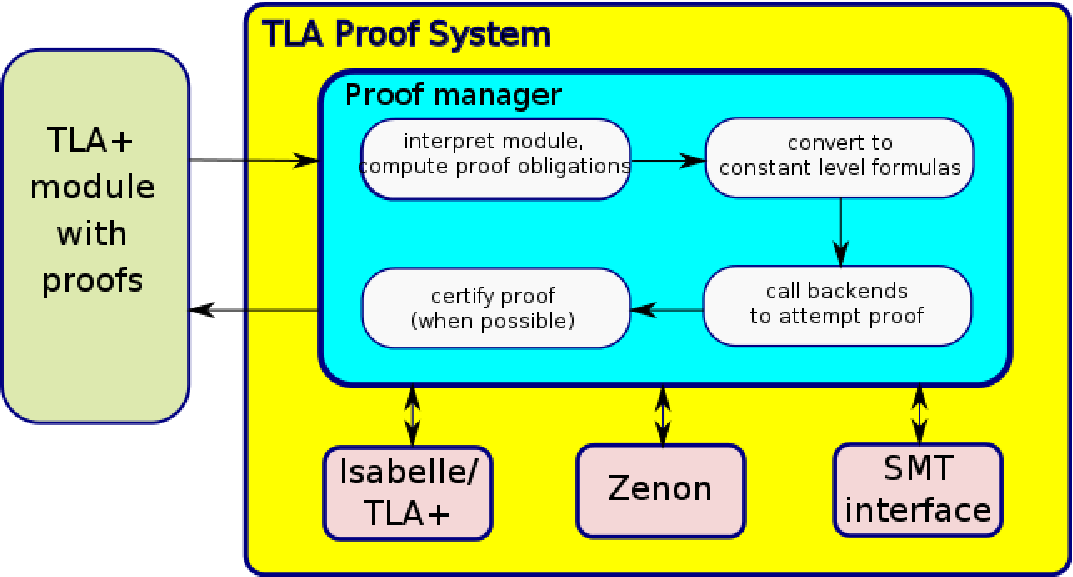
\includegraphics[width=1.0\linewidth]{architecture}}
\end{frame}

\begin{frame}
  \frametitle{Proof Manager}

  \begin{itemize}
  \item \tc{dkblue}{Interpret \tlaplus\ proof language}

    \begin{itemize}
    \o interpret module structure (imports and instantiations)
    \o manage context: known and usable facts and definitions
    \o expand operator definitions if they are usable
    \end{itemize}

  \oo \tc{dkblue}{Rewrite proof obligations to constant level}

    \begin{itemize}
    \o handle primed expressions such as\ \ \tc{dkgreen}{$Inv'$}
    \o distribute prime over (constant-level) operators
    \o introduce distinct symbols \tc{dkgreen}{$e$} and \tc{dkgreen}{$e'$}
       for atomic state expression \tc{dkgreen}{$e$}
    \end{itemize}

  \oo \tc{dkblue}{Invoke backend provers}

    \begin{itemize}
    \o user may explicitly indicate which proof method to apply
    \o optionally: certify backend proof
    \end{itemize}
  \end{itemize}
\end{frame}

%%% Local Variables: 
%%% mode: latex
%%% TeX-master: "tutorial"
%%% End: 

\section{Hints on Using the Prover Effectively}

\begin{frame}
  \frametitle{Control the Size of Formulas}

  \begin{itemize}
  \item \tc{dkblue}{Proof obligations are often large}

    \begin{itemize}
    \o long definitions of actions and invariants
    \o \kw{let} constructions add to complexity when expanded
    \end{itemize}

  \oo \tc{dkblue}{The backend provers are easily overwhelmed by large formulas}

    \begin{itemize}
    \o may work on top-level operators or deeply inside a long formula
    \o even simple proof steps may take an extraordinate amount of time
    \end{itemize}

  \oo \alert{Use local definitions and \HIDE\ them when unnecessary}

    \begin{itemize}
    \o prove facts about a \kw{let}-bound operator, then \HIDE\ it
    \end{itemize}
  \end{itemize}

  \vfill\vfill
\end{frame}

\begin{frame}
  \frametitle{Example: Controlling the Size of Expressions}

  \qquad\begin{tlablock}
    \LEMMA\
    \begin{noj2}
      & \begin{conj}
          x \in SomeVeryBigExpression\\
          y \in AnotherBigExpression
        \end{conj}\\
      \biimplies &
        \begin{conj}
            y \in AnotherBigExpression\\
            x \in SomeVeryBigExpression
        \end{conj}
\pause
        \hspace{1cm}\raisebox{0cm}[0pt][0pt]{\begin{minipage}{3cm}
          \begin{beamercolorbox}[rounded=true,shadow=true]{postit}\footnotesize
            \OBVIOUS\ may take\\forever here
          \end{beamercolorbox}
        \end{minipage}}
    \end{noj2}\\
\pause
    \ps{1}{.}\ \ \ \DEFINE\ S\ \deq\ SomeVeryBigExpression\\
    \ps{1}{.}\ \ \ \DEFINE\ T\ \deq\ AnotherBigExpression\\
    \ps{1}{1.}\ S = SomeVeryBigExpression\\
    \quad\OBVIOUS\\
    \ps{1}{2.}\ T = AnotherBigExpression\\
    \quad\OBVIOUS\\
    \ps{1}{.}\ \ \ \HIDE\ \DEF\ S,\ T\\
    \ps{1}{3.}\ 
      \begin{noj2}
        & x \in S \land y \in T\\
        \biimplies & y \in T \land x \in S
      \end{noj2}\\
    \quad\OBVIOUS\\
    \ps{1}{4.}\ \QED\qquad\BY\ \ps{1}{1},\ \ps{1}{2},\ \ps{1}{3}
  \end{tlablock}
\end{frame}

\begin{frame}
  \frametitle{Avoid Circular Rewrites}

  \begin{itemize}
  \item \tc{dkblue}{Rewriting is often effective for reasoning about equalities}

    \begin{itemize}
    \o idea: replace left-hand side of equality by right-hand side
    \o Isabelle's automatic tactic are based on rewriting
    \o for example, use\ \ \tc{dkgreen}{$x' = x-y \land y'=y$}\ \ to eliminate $x'$ and $y'$    \end{itemize}

\pause

  \oo \tc{dkblue}{Must make sure that rewriting terminates}

    \begin{itemize}
    \o consider\ \ \tc{dkgreen}{$s = f(t) \land t = g(s)$}
    \o Isabelle attempts to reject circular sets of equations
    \o if rejected, proof may get stuck
    \o if not rejected, proof may never terminate
    \end{itemize}

  \oo \alert{Use local definitions, and \HIDE\ them to break loops}
  \end{itemize}
\end{frame}

\begin{frame}
  \frametitle{Circular Rewrites: Example}

  \qquad\begin{tlablock}
    \ps{4}{5.}\ r.name = \str{xyz}\\
    \quad\ps{5}{1.}\ r = [name \mapsto "xyz",\ value \mapsto \alt<1>{r}{\alert{r}}.value]\\
    \quad\quad\BY\ \ps{2}{2}\\
    \quad\ps{5}{2.}\ \QED\\
    \quad\quad\BY\ \ps{5}{1}
  \end{tlablock}

\pause

  \vfill\vfill

  \qquad\alert{The equation in step $\ps{5}{1}$ is circular!}

  \vfill\vfill

\pause

  \qquad\begin{tlablock}
    \ps{4}{5.}\ r.name = \str{xyz}\\
    \quad\ps{5}{}\ \ \ \DEFINE\ rval\ \deq\ r.value\\
    \quad\ps{5}{1.}\ r = [name \mapsto "xyz",\ value \mapsto rval]\\
    \quad\quad\BY\ \ps{2}{2}\\
    \quad\ps{5}{}\ \ \ \HIDE\ \DEF\ rval\\
    \quad\ps{5}{2.}\ \QED\\
    \quad\quad\BY\ \ps{5}{1}
  \end{tlablock}
\end{frame}

\begin{frame}
  \frametitle{Establishing Facts About \CHOOSE}

  \qquad\begin{tlablock}
    \DEFINE\ m\ \deq\ \CHOOSE x \in S : P(x)\\
    \DEFINE\ NoValue\ \deq\ \CHOOSE x : x \notin Value
  \end{tlablock}

  \begin{itemize}
  \oo \tc{dkblue}{How to prove a property $Q(m)$ ?}

    \begin{itemize}
    \o \CHOOSE\ always denotes some value, even if $P(x)$ holds for no $x \in S$
    \end{itemize}

\pause

  \oo \tc{dkblue}{In practice, must establish the two following facts}

    \begin{itemize}
    \o $\E x \in S : P(x)$
    \o $\A x \in S : P(x) \implies Q(x)$
    \o \tlaps\ will then deduce $Q(m)$
    \end{itemize}

\pause

  \oo \tc{dkblue}{Important special case: ``null'' values}

    \begin{itemize}
    \o existence of such a value follows from the library theorem

      \medskip

      \begin{tlablock}
        NoSetContainsEverything\ \deq\ \A S : \E x : x \notin S
      \end{tlablock}
    \end{itemize}
  \end{itemize}
\end{frame}

\begin{frame}
  \frametitle{It's Easier To Prove Something If It's True}

  \begin{itemize}
  \item \tc{dkblue}{All specifications initially contain mistakes}

    \begin{itemize}
    \o errors range from typos to misunderstandings to genuine bugs
    \o formal mathematical definitions are hard to get right
    \end{itemize}

  \oo \tc{dkblue}{\tlaps\ is not good at catching specification errors}

    \begin{itemize}
    \o if you are stuck on a proof, is it you, the prover or the specification?
    \o even with structured proofs, complexity quickly gets out of hand
    \end{itemize}

  \oo \tc{dkblue}{Extensively debug your specifications using \tlc}

    \begin{itemize}
    \o almost all bugs manifest themselves on small instances
    \o run \tlc\ on many properties and inspect the counter-examples
    \end{itemize}
  \end{itemize}
\end{frame}

\begin{frame}
  \frametitle{Focus On The Theorems You Are Interested In}

  \begin{itemize}
  \item \tc{dkblue}{\tlaps\ currently has limited support for theories}

    \begin{itemize}
    \o set theory and functions are fully supported
    \o decision procedure for elementary integer arithmetic
    \o very rudimentary support for sequences
    \end{itemize}

\pause

  \oo \tc{dkblue}{State facts about ``data'' as assumptions}

    \begin{itemize}
    \o do you want to verify an algorithm or basic mathematics?
    \o but --- isn't that dangerous?
    \o it is, but you can validate many assumptions using \tlc
    \o override infinite sets with finite ones in the model, e.g.\ \ \tc{dkgreen}{$Nat\ \deq\ 0..50$}
    \end{itemize}

\pause

  \oo \alert{Theory support will improve slowly and your help is welcome}
  \end{itemize}
\end{frame}

%%% Local Variables: 
%%% mode: latex
%%% TeX-master: "tutorial"
%%% End: 


\section{Case Study: Peterson's Algorithm}

\end{document}

%%% Local Variables: 
%%% mode: latex
%%% TeX-master: t
%%% End: 
